\documentclass[11pt]{scrartcl}
\usepackage{booktabs}
\usepackage{bbding}
\usepackage{settings}

\lhead{\today}
\rhead{\begin{CJK}{UTF8}{ipxm} カズマアカリ。
\end{CJK}}
\usepackage{pdfpages}
\begin{document}

\title{\vspace{-2em}\textcolor{bk}{\textbf{BÀI TẬP TỔ HỢP VÀ ĐẠI SỐ}}}

%\subtitle{\vspace{1.5em}{\textbf{\LARGE CAUCHY-SCHWARZ-HOLDER}}}
\author{Phạm Bảo -\begin{CJK}{UTF8}{ipxm} カズマアカリ。\end{CJK}\vspace{-1em}}


%\maketitle
\thispagestyle{empty}

\tableofcontents
\newpage
%\subsection*{\Large\textcolor{bk}{ \S 1.1.} Các bất đẳng thức cổ điển}


\setcounter{page}{1}
\thispagestyle{plain}
\begin{itemize}[label=, leftmargin=0em, itemsep=0.5em]
    
    \section{\huge Dãy số}
    \subsection{\LARGE \textcolor{dk}{Đề bài}}
    
    \item \begin{bt}\vocab{(Đồng Nai TST 2023).}
        Cho dãy số $(a_n)$ thỏa mãn $a_1 = 1$ và $$a_{n + 1} = \sqrt{2n + a_n^2 + \frac{1}{a_n}}, n \geq 1$$.
        \begin{enumerate}[label=(\alph*)]
            \item Chứng minh rằng $a_n \leq n$, với mọi số nguyên dương $n$.
            \item Tìm $\dlim a_n$
        \end{enumerate}
    \end{bt}
    \begin{sol}
        (a) Thật vậy, bằng quy nạp ta dễ dàng chứng minh được $a_n \geq 1, \forall n \geq 1$. Khi này, giả sử $a_{n} \leq n$, ta có 
        \[
            a_{n + 1} = \sqrt{2n + a_n^2 + \frac{1}{a_n}} \leq \sqrt{2n + n^2 + 1 } = \sqrt{(n + 1)^2} = n + 1
        \]
        hoàn tất chứng minh.

        (b) Ta có 
        \(
        a_{n + 1} \geq \sqrt{2n + 1 + \frac{1}{n}} 
        \). Cho $n \to +\infty$ thì ta được $\dlim a_n = +\infty$.
    \end{sol}
    \item \begin{bt}\vocab{(Hà Tĩnh TST 2023).}
        Cho dãy số $(u_n)$ xác định bởi $u_1 = 1$ và $$u_{n + 1} = 1 + \frac{1}{u_n + 1}, n \geq 1$$
        \begin{enumerate}[label=(\alph*)]
            \item Chứng minh rằng dãy số $(u_n)$ có giới hạn hữu hạn và tìm giới hạn đó.
            \item Chứng minh rằng $\dsum_{i = 1}^n u_i^2 < 2n, n \geq 1$.
        \end{enumerate}
    \end{bt}
    \begin{sol}
        (a) Ta cần chứng minh $\sqrt{2} \leq u_n \leq \frac{3}{2}, \forall n \geq 2$ bằng quy nạp. Với $n = 2$ thì rõ ràng luôn đúng, giả sử với $n\geq 2$ ta có $\sqrt{2} < u_{n} \leq \frac{3}{2}$, khi đó 
        \[
            u_{n + 1} = 1 + \frac{1}{u_n + 1} \leq 1 + \frac{1}{\sqrt{2} + 1}  \leq \frac{3}{2}
        \]
        \[
            u_{n + 1} = 1 + \frac{1}{u_n + 1} \geq 1 + \frac{1}{\frac{3}{2} + 1} > \sqrt{2}
        \]
        Khi này có đánh giá 
        \[
        |u_{n + 1} - \sqrt{2}| = \left|\frac{u_{n} + 2}{u_n + 1} -\sqrt{2}\right| \leq \left|\frac{u_n + 2}{\sqrt{2} + 1} - \sqrt{2}\right| = \frac{\left|u_n - \sqrt{2}\right|}{\sqrt{2} + 1} =\dots = \frac{1}{(\sqrt{2} + 1)^n}|u_1 -\sqrt{2}|
        \]
        Khi này tồn tại $N_0$ đủ lớn để $\forall n > N_0$ thì $\frac{1}{(\sqrt{2} + 1)^n}|u_n -\sqrt{2}| < \varepsilon \ra |u_{n + 1} - \sqrt{2}| < \varepsilon, \forall n > N_0$, suy ra $\dlim u_n = \sqrt{2}$.

        (b) Với chú ý $u_{n} > \sqrt{2},\forall n\geq 1$, ta có 
        \[
        \begin{aligned}
            \sum_{i = 1}^n u_i^2 = 1 + \sum_{i = 1}^{n - 1} \left(1 + \frac{1}{u_i+ 1}\right)^2 &= 1 + \sum_{i = 2}^{n - 1}1 + \frac{2}{u_i + 1} + \frac{1}{(u_i + 1)^2}\\
            &< 1  + \left(n -1 \right)\left(\frac{2}{\sqrt{2} + 1} + \frac{1}{(\sqrt{2} + 1)^2}\right)\\
            &=1 + (n - 1) = n
        \end{aligned}
        \]
        Chứng minh hoàn tất.
    \end{sol}
    \item \begin{bt}\vocab{(Hà Nội TST 2022).}
        Cho dãy $(x_n)$ được xác định bởi $x_1 = x_2 = 1$ và $x_{n + 2} = x_{n + 1}^2 - \frac{1}{3}x_n$ với $n \geq 1$. Chứng minh rằng $(x_n)$ có giới hạn hữu hạn và tìm giới hạn đó.
    \end{bt}
    \begin{sol}
        Ta có thể dự đoán rằng $\dlim x_n = 0$. Ta sẽ chứng minh $|x_n| < \frac{1}{3}$ bằng quy nạp. Với $n =4,5$ thì rõ ràng thỏa mãn, giả sử với $|x_{k}| < \frac{1}{3}, \forall 5 <k < n$.
        
        Khi đó ta có $|x_{n + 2}| < |x_{n + 1}^2| + \frac{1}{3}|x_n| < \frac{1}{3^2} + \frac{1}{3}.\frac{1}{3} < \frac{1}{3}$. Vậy nên từ đây ta được 
        \[
         |x_{n + 2}| < \frac{1}{3}|x_{n + 1}| + \frac{1}{3}|x_n|
        \]
        Theo bổ đề dãy số ta được $\dlim x_n = 0$.
    \end{sol}
    \item \begin{bt}\vocab{(PTNK 2023).}
        Cho dãy $(u_n)$ thỏa mãn $u_1 = 1$ và $u_{n + 1} = u_n + \frac{\ln n}{u_n}, n \geq 1$.
        \begin{enumerate}[label=(\alph*)]
            \item Chứng minh rằng $u_{2023} > \sqrt{2023 \ln 2023}$
            \item Tìm $\dlim\frac{u_n  \ln n}{n}$.
        \end{enumerate}
    \end{bt}
    \begin{sol}
        (a) Ta sẽ chứng minh $u_n >\sqrt{n\ln n}, \forall n > 4$ bằng quy nạp. Với $n = 5$ thì dễ dàng kiểm tra đúng, giả sử với $n - 1 > 4$ ta có $u_{n} > \sqrt{n\ln n}$. Sử dụng bất đẳng thức AM-GM ta có $u_{n + 1} \geq 2\sqrt{\ln(n)}$. Xét $f(x) = x + \frac{\ln(n)}{x}$ trên $[2\sqrt{\ln(n)}, +\infty)$ ta có 
        \[
            f'(x) = 1 - \frac{\ln(n)}{x^2} \geq 1 - \frac{\ln(n)}{4\ln(n)} = > 0
        \]
        Suy ra $f$ là hàm tăng ngặt. Khi đó
        \[
            u_{n + 1} = f(u_n) > f(\sqrt{n\ln(n)}) = \sqrt{n\ln(n)} + \frac{\ln(n)}{\sqrt{n\ln(n)}}
        \]
        Ta cần chứng minh $\sqrt{n\ln(n)} + \frac{\ln(n)}{\sqrt{n\ln(n)}} \geq \sqrt{(n + 1)\ln(n + 1)}$.

        Xét $g(x) = \sqrt{x\ln(x)}$ trên $[n, n+ 1]$ có 
    \end{sol}
    \item \begin{bt}\vocab{(Trại hè Hùng Vương 2023).}
        Cho dãy số $(u_n)$ được xác định bởi $u_1 = 3$ và $$u_{n + 1} = u_n^2 + u_n - 4, n \geq 1$$ Tìm $\dlim\frac{(u_1 + 1)(u_2 + 3)\dots(u_n + 3)}{u_{n + 1} +3}$.
    \end{bt}
    \begin{sol}
        Bằng quy nạp, ta dễ dàng chứng minh được $u_n > 2, \forall n \geq 1$. Ta có 
        \[
            u_{n + 1} - 2 = (u_n - 2)(u_n + 3) \lra u_n + 3 = \frac{u_{n + 1} - 2}{u_n - 2}
        \]
        Cho nên từ đây viết lại $\dprod_{i = 1}^n (u_i + 3) = \dprod_{i = 1}^n \frac{u_{i + 1} - 2}{u_i - 2} = \frac{u_{n + 1} - 2}{3- 2} = u_{n + 1} - 2$. Mặt khác, bằng Weierstrass ta dễ dàng chứng minh được $\dlim u_n = +\infty$, nên từ đó tính được \[\dlim\frac{(u_1 + 1)(u_2 + 3)\dots(u_n + 3)}{u_{n + 1} +3} = \dlim \frac{u_n - 2}{u_n + 3} = 1\]
    \end{sol}

    
    \item \begin{bt}\vocab{(Bình Phước TST 2023).}
        Cho đãy số $\left(a_n\right)$ xác định bởi: \[\left\{\begin{array}{l}a_1=\frac{2024}{2023} \\ a_{n+1}=a_n+2 \sqrt{a_n}+\frac{n^2}{a_n}, \forall n \geq 1 .\end{array}\right.\]
        \begin{enumerate}[label=(\alph*)]
            \item Chứng minh rằng dãy số $\left(b_n\right)$ xác định bởi $b_n=\dsum_{i=1}^n \frac{1}{a_i}$ có giới hạn hữu hạn.
            \item Xét dãy số $\left(c_n\right)$ xác định bởi $c_n=\left[\dsum_{i=1}^n \frac{i}{a_i}\right]$.Chứng minh rằng mỗi số nguyên dương đều xuất hiện trong dãy $\left(c_n\right)$.
        \end{enumerate}
        
    \end{bt}
    \begin{sol}

        (a) Ta chứng minh quy nạp $n^2 \leq a_n \leq (n + 1)^2, \forall n \geq 1$. Với $n = 1$ thì dễ dàng kiểm tra, giả sử với $n > 1$ nào đó ta có $n^2 \leq a_n \leq (n +1)^2$, ta xét hàm số $f(x) = x + 2\sqrt{x} + \frac{n^2}{x}$ trên đoạn $[n, +\infty)$. Ta có $f'(x) = 1 + \frac{1}{\sqrt{x}} - \frac{n^2}{x^2} \geq 1 + \frac{1}{x} - 1 \geq 0$, suy ra $f(x)$ là hàm tăng, vậy nên ta được 
        \[
        a_{n + 1} = f(a_n) \leq f((n + 1)^2) = (n + 1)^2 + 2(n + 1) + \frac{n^2}{(n + 1)^2} \leq (n + 2)^2
        \]
        Hơn nữa 
        \[
        a_{n + 1} = f(a_n) \geq f(n^2) = n^2 + 2n + 1 = (n + 1)^2
        \]
        Hoàn tất quy nạp. Khi đó 
        \[
            b_n = \dsum \frac{1}{a_i} \leq \dsum \frac{1}{(i + 1)^2} < 2
        \]
        Vì $(b_n)$ tăng và bị chặn nên $(b_n)$ hội tụ
        
        (b) 
        Ta có một bổ đề sau 
        \begin{theo}[Bổ đề quan trọng]
            -Cho một dãy số thực $(a_n)$ thỏa mãn $0 < a_n \leq 1, \forall n \geq 1$ và $\dlim \dsum_{i = 1}^n a_n = +\infty$. Khi đó với mọi số nguyên dương $M$, luôn tồn tại $N > 0$ để với $n_0 > N$ nào đó thì 
            \[
            \left\lfloor \dsum_{i = 1}^{n_0} a_i \right\rfloor = M
            \]
        \end{theo}
        \begin{proof} Ta sẽ chứng minh bổ đề này bằng phản chứng. Đặt $b_n = \dsum_{i = 1}^n a_n$. Giả sử không tồn tại $N_0$ để thỏa mãn bổ đề, khi đó sẽ có hai trường hợp xảy ra. 

        \vocab{Trường hợp 1:} Không tồn tại $n_0$ để $\lfloor b_{n_0}\rfloor =M$ mà lại tồn tại $m_0$ để $\lfloor b_{m_0} \rfloor > M$. Để $(\lfloor b_n \rfloor)$ không nhận giá trị của $M$ mà lại nhận những giá trị nguyên lớn hơn nó thì phải tồn tại $a_k$ để $a_k > 1$, điều này là vô lý.

        \vocab{Trường hợp 2: } Không tồn tại $n_0$ để $\lfloor b_{n_0}\rfloor =M$ và cũng không tồn tại $m_0$ để $\lfloor b_{m_0} \rfloor > M$. Khi này rõ ràng là đến một lúc nào đó, sẽ tồn tại $m > 0$ và $N > 0$ để $b_{n_0} < m, \forall n_0 > N$, tức là $(b_n)$ bị chặn trên. Mặt khác $(b_n)$ cũng là dãy tăng, nên theo Weierstrass thì $(b_n)$ có giới hạn hữu hạn, cũng vô lý. 

        Vậy là bổ đề đã được chứng minh.
        \end{proof}
        Mặt khác, ta có 
        \[
            \dsum_{i = 1}^n \frac{i}{a_i} \geq \dsum_{i = 1}^n \frac{i}{(i + 1)^2} = \dsum_{i = 2}^n \frac{1}{i} - \dsum_{i = 1}^{n} \frac{1}{i^2} > \dsum_{i = 2}^n \frac{1}{i} - 2
        \] Cho $n \to +\infty$ thì ta được $\dlim s_n = +\infty$. Khi đó, áp dụng bổ đề trên, ta có được điều phải chứng minh.
        
        

        
    \end{sol}
    \item \begin{bt}\vocab{(PTNK 2022).}
        Cho dãy số $(u_n)$ được xác định bởi $u_1 = 1$ và $u_{n + 1} = \sqrt{2 + u_n}, n \geq 1$. Tính
        \[
            \lim_{n \to + \infty} \frac{1}{\ln n}\left(\frac{u_1}{1} + \frac{u_2}{2} + \dots + \frac{u_n}{n}\right)
        \]
    \end{bt}
    \begin{sol}
        Đặt $u_1 = 2\cos\frac{\pi}{3}$, có $u_2 = \sqrt{2 + 2\cos\frac{\pi}{3} }= 2\cos\frac{\pi}{3.2}$. Bằng quy nạp, ta chứng minh được $u_n = 2\cos\frac{\pi}{3.2^{n - 1}}$. Theo định lý Stolz, ta có 
        \[
            \lim_{n \to + \infty} \frac{\frac{u_1}{1} + \frac{u_2}{2} + \dots + \frac{u_n}{n}}{\ln n } = \dlim \frac{\frac{u_{n + 1}}{n + 1}}{\ln(n + 1) - \ln(n)} = \dlim \frac{2\cos\frac{\pi}{3.2^{n - 1}}}{\ln\left(1 + \frac{1}{n}\right)^{n + 1}} = 2
        \]
        Vậy nên $\dlim \frac{1}{\ln n}\left(\frac{u_1}{1} + \frac{u_2}{2} + \dots + \frac{u_n}{n}\right) = 2$.
    \end{sol}

    \item \begin{bt}\vocab{(Kon Tum TST 2023).} Cho các ý sau:
        \begin{enumerate}
            \item Cho dãy số $(u_n)$ được xác định bởi
            \[\left\{
                \begin{array}{l}
                    u_1 = 2 \\
                    u_n = u_{n - 1} + 2n + 3, \forall n \geq 1 
                \end{array}\right.\]
            Chứng minh rằng $u_n + 7$ là số chính phương với mọi $n \geq 1$.
            
            \item Cho dãy số $(u_n)$ được xác định bởi
            \[\left\{
                \begin{array}{l}
                    u_1 = 2023\\
                    u_{n + 1} = \frac{u_n^2 + 8}{2(u_n - 1)}, \forall n \geq 1
                \end{array}
            \right.
            \]
            Chứng minh dãy $(u_n)$ có giới hạn hữu hạn và tìm giới hạn đó.
        \end{enumerate}
    \end{bt}
    \begin{sol}
        1. Ta xét tổng như sau:
        \[
            \begin{aligned}
                u_n &= u_{n - 1} + 2n + 3\\
                    &= u_{n - 2} + 2n + 3 + 2(n - 1) + 3\\
                    &=\dots\\
                    &= \dsum_{i = 2}^n 2i + 3  + 2\\
                    &= 3n - 3 + 2 + n(n + 1)  - 2\\
                    &= n^2 + 4n - 3\\
            \end{aligned}
        \]
        Khi đó $u_n + 7 = (n + 2)^2, \forall n \geq 1$ là số chính phương.

        2. Ta có 
        \[
            u_{n + 1} - 4 = \frac{u_n^2 + 8 - 8u_n +8}{2(u_n - 1)} = \frac{(u_n - 4)^2}{2(u_n - 1)}
        \]
        \[
            u_{n + 1} + 2 = \frac{u_n^2 + 8 + 4u_n - 4}{2(u_n - 1)} = \frac{(u_n + 2)^2}{2(u_n - 1)}
        \]
        Từ đây suy ra 
        \[
            \frac{u_{n + 1} - 4}{u_{n + 1} + 2} = \left(\frac{u_n - 4}{u_n + 2}\right)^2 = \left(\frac{u_{n - 1} - 4}{u_{n - 1}+ 2}\right)^{2.2} = \dots = \left(\frac{u_1 - 4}{u_1 + 2}\right)^{2^n} = \left(\frac{2019}{2025}\right)^{2^n}
        \]
        Đặt $k_n = \left(\frac{2019}{2025}\right)^{2^n}$. Tương dương với 
        \[
        1 - \frac{6}{u_{n + 1} + 2} = k_n \lra u_{n + 1} = \frac{6}{1 - k_n} - 2
        \]
        Cho $n \to +\infty$ thì $k_n \to 0$, từ đó ta được $\dlim u_n = 4$.
    \end{sol}
    \item \begin{bt}\vocab{(Sóc Trăng TST 2023).} Với số thực $a$, xét dãy số $(u_n)$ xác định bởi
    \[
        u_1 = a \text{ và } u_{n + 1} = \frac{u_n^2}{2 - u_n^2}, n \geq 1
    \]
    \begin{enumerate}
        \item Chứng minh rằng với mọi $a$ hữu tỷ, các số hạng của $(u_n)$ luôn xác định.
        \item Với $a \in [0,1]$, chứng minh rằng dãy số $(v_n)$ xác định bởi $v_n = n^2 u_n$ luôn có giới hạn hữu hạn và xác định giới hạn đó.
    \end{enumerate}
    \end{bt}
    \begin{sol}
        
        1. Vì $a$ hữu tỉ nên $u_n \in \bb{Q}, \forall n \geq 1$. Khi đó $2 - u_n^2 \neq 0$ vì $u_n \neq \pm\sqrt{2}, \forall n \geq 1$. Vậy nên mọi số hạng của $(u_n)$ luôn xác định.

        2. Bằng quy nạp ta chứng minh được $0 \leq u_n \leq 1, \forall n \geq 1$. Lại có 
        \[
            \frac{u_{n + 1}}{u_n} = \frac{u_n}{2 - u_n^2} \leq \frac{1}{2 - 1} = 1
        \]
        Suy ra $(u_n)$ giảm và bị chặn dưới nên $(u_n)$ hội tụ. Giải phương trình giới hạn tìm được $\dlim u_n = 0$. Theo định lý Stolz-Cesaro ta có 
        \[
        \dlim \frac{1}{n\sqrt{u_n}} = \dlim \frac{1}{\sqrt{u_{n + 1}}} - \frac{1}{\sqrt{u_n}} = \dlim \frac{\sqrt{2 - u_n^2}}{u_n} - \frac{1}{\sqrt{u_n}}= \blim_{x \to 0} \frac{\sqrt{2 - x^2} - \sqrt{x}}{x} = +\infty
        \]
        Vậy nên $\dlim v_n = \dlim n^2u_n = 0$.
    \end{sol}
    \begin{bt}\vocab{(Thanh Hóa TST 2023).} Cho dãy số $(u_n)$ được xác định bởi
        \[
            x_1 = \frac{1}{2} \text{ và } x_{n + 1} = \frac{1}{4} \left(x_n + \frac{3}{x_n}\right), n \geq 1
        \]
    Chứng minh rằng dãy số $(x_n)$ có giới hạn hữu hạn và tính giới hạn đó.
    \end{bt}
    \begin{sol}
        Sử dụng bất đẳng thức AM-GM ta có $x_{n + 1} \geq \frac{\sqrt{3}}{2},\forall n \geq 1$. Ta chứng minh $x_n < 2, \forall n \geq 1$. Với $n = 1$ thì dễ dàng kiểm tra, giả sử có $x_n < 2$. Ta có
        \[
        x_{n + 1} \leq \frac{2}{4} + \frac{3.2}{4.\sqrt{3}} <2
        \]
        Suy ra $x_n \in (\frac{\sqrt{3}}{2},2)$. Ta có 
        \[
            x_{n +1} - x_n = \frac{3}{4}\left(\frac{1}{x_n} - x_n\right) > \frac{3}{4}\left(   \frac{2}{\sqrt{3}} - \frac{\sqrt{3}}{2} \right) > 0
        \]
        Suy ra $(x_n)$ tăng và bị chặn trên nên có giới hạn. 
        
        Giải phương trình giới hạn tìm được $\dlim x_n = 1$.
    \end{sol}
    \item \begin{bt}\vocab{(Tiền Giang TST 2023).}
        Cho dãy số $(a_n)$ được xác định bởi
        \[
            0 < a_1 \neq 1 \text{ và } a_{n + 1} = a_n + \frac{n}{a_n}, n \geq 1 
        \]
        \begin{enumerate}[label=(\alph*)]
            \item Chứng minh rằng $a_n > n, \forall n \geq 2$
            \item Tính $\dlim (a_n - n)$
        \end{enumerate}
    \end{bt}
    \begin{sol}

        (a) Sử dụng bất đẳng thức AM-GM ta có $a_{n + 1} \geq 2\sqrt{n}$. Xét $f(x) = x + \frac{n}{x}$ trên $[2\sqrt{n - 1},+\infty)$. Ta có $f'(x)= 1 - \frac{n}{x^2} \geq 1 - \frac{n}{4n - 4} > 0$. Do đó $f$ là hàm tăng ngặt. 
        
        Ta chứng minh $a_n > n, \forall n \geq 2$ bằng quy nạp. Với $n = 2$ thì $a_2 = a_1 + \frac{2}{a_1} > 2$. Giả sử với $n > 2$ thì $a_n > n$, khi đó 
        \[
            a_{n + 1} = f(a_n) > f(n) = n + 1
        \]
        Vậy $a_n > n, \forall n \geq 2$.

        (b) Đặt $u_n = a_n - n$ khi đó viết lại 
        \[
            u_{n + 1}  = u_n - 1 + \frac{n}{u_n + n}, \forall n \geq 1
        \]
        Khi đó có 
        \[
            u_{n + 1} - u_n = -1 + \frac{n}{u_n +n} < -1 + 1 = 0
        \]
        Mặt khác để ý rằng $u_n > 0, \forall n \geq 1$ suy ra $u_n$ là dãy giảm và bị chặn dưới nên $(u_n)$ hội tụ. Đặt $\dlim u_n = \lambda$, cho $n \to +\infty$ ta được 
        \[
            \lambda = \lambda - 1 + \frac{1}{\lambda} \ra \lambda = 1
        \]
        Vậy $\dlim u_n = \dlim (a_n - n) = 1$.
    \end{sol}
    \item \begin{btvn}\vocab{\href{https://youtu.be/jsNmOM8S2po?si=H-oE95ze7Y6XjSO7}{(TST Phú Yên 2023).}}
        Cho hai dãy số $(u_n)$ và $(v_n)$ được xác định bởi
        \[
            \left\{
                \begin{array}{l}
                    u_1 = 4, v_1 = 2\\
                    u_{n + 1} = u_n^2 + 3v_n\\
                    v_{n + 1} =2u_nv_n
                \end{array}
            \right.
        \]
        Tìm $\displaystyle \lim_{n \to +\infty}\sqrt[2^n]{v_n}$ và $\displaystyle \lim_{n \to +\infty}\sqrt[2^n]{u_1u_2\dots u_n}$.
    \end{btvn}
    \item \begin{btvn}\vocab{\href{https://youtu.be/gqwfWR4fmEQ?si=M_6OgMGvI4iS9jHL}{(TST Quảng Bình 2023).}}
        Cho hai dãy số $(u_n)$ và $(v_n)$ được xác định bởi
        \[
            \left\{
                \begin{array}{l}
                    u_1 = 2024\\
                    (n + 1)^2u_{n + 1} =(n^2 + 2n)u_n + 2023, n \geq 1
                \end{array}
            \right.
        \]
        Tìm giới hạn của dãy số $(u_n)$.
    \end{btvn}
    \item \begin{btvn}\vocab{\href{https://youtu.be/3gCwGsteyO0?si=R2vB3_TBLXd6PYSw}{(Epsilon).}}
        Cho dãy số $\left(x_n\right)_{n=1}^{+\infty}$ như sau: $x_1=a>2$ và
            $$
            x_{n+1}=x_n^2-2, \forall n=1,2, \ldots
            $$
            Tính $\displaystyle\lim _{n \rightarrow+\infty}\left(\frac{1}{x_1}+\frac{1}{x_1 x_2}+\frac{1}{x_1 x_2 x_3}+\cdots+\frac{1}{x_1 x_2 \ldots x_n}\right)$.
    \end{btvn}
    \item \begin{btvn}\vocab{\href{https://youtu.be/3gCwGsteyO0?si=R2vB3_TBLXd6PYSw}{(Hà Tĩnh 2014).}}
        Cho dãy số $\left(u_n\right)$ thỏa mãn:
        $$
        \left\{\begin{array}{l}
        u_1=1 ; u_2=3 \\
        \frac{u_{n+1}}{u_n}=\frac{u_n^2}{u_{n-1}^2}-2, n \geq 1 .
        \end{array}\right.
        $$

        Chứng minh $\frac{1}{u_1}+\frac{1}{u_2}+\ldots+\frac{1}{u_n}<\frac{5-\sqrt{5}}{2}$ với mọi $n \geq 1$.
    \end{btvn}
    \item \begin{btvn}\vocab{(Gặp gỡ toán học 2010).}
        Cho dãy số $(x_n)$ được xác định bởi
        \[
            x_1 = 1, x_{n + 1} = x_n + \frac{1}{x_n}, \forall n \geq 1
        \]
        \begin{enumerate}
            \item Chứng minh rằng $\dlim x_n = +\infty$
            \item Tìm $\lim_{n \to +\infty}\frac{x_n}{\sqrt{n}}$.
        \end{enumerate}
    \end{btvn}
    \item \begin{btvn}\vocab{\href{https://youtu.be/PITrGXRwWgk?si=48dpyJynXmDHQDFs}{(Đồng Nai 2022).}}
        Cho dãy số dương $(u_n)$ được xác định bởi \[u_0 = 2, u_1 = 4 \text{ và } u_{n + 2} =2\sqrt{4u_{n + 1}^2 - u_nu_{n + 2}} + u_n\text{ với } n \geq 1\]
        \begin{enumerate}[label=(\alph*)]
            \item Tìm công thức tổng quát của $(u_n)$.
            \item Với mỗi số nguyên dương $n$. Đặt $S_n = \dsum_{i = 0}^n \frac{1}{u_i}$. Chứng minh rằng $(S_n)$ có giới hạn hữu hạn và tìm giới hạn đó.
        \end{enumerate}
    \end{btvn}
    \item \begin{btvn}\vocab{\href{https://youtu.be/gm3A3g_USIM?si=kokHTJ8RcjuvD2QJ}{(Epsilon).}}
        Cho dãy $(u_n)$ được xác định bởi 
        \[
            u_1 = 1, u_2 = 2, ( n + 1)u_{n + 2} = n(u_{n + 1} + u_n) + 2\left(u_{n + 1} + \frac{u_n}{n}\right) + 3u_n, \text{ với } n\geq 1 
        \]
        Chứng minh rằng dãy $\left(\frac{u_{n + 1}}{u_n}\right)_{n \geq 1}$ có giới hạn hữu hạn và tìm giới hạn đó.
    \end{btvn}
    \item \begin{btvn}\vocab{\href{https://youtu.be/ZkFer1ma5Ew?si=lX8buOq2Q-JVIyZG}{(Epsilon).}}
        Cho dãy số $(x_n)$ được xác định bởi $x_1 = 1$ và 
        \[
            x_{n + 1} = \frac{x_1}{n + 1} + \frac{x_2}{n + 2} +\dots+ \frac{x_n}{2n}, n \geq 1
        \]
        Chứng minh rằng $(x_n)$ có giới hạn hữu hạn và tìm giới hạn đó.
    \end{btvn}

    \begin{bt}\vocab{\href{https://youtu.be/pzwR1_D3TP8?si=eRida3THH4oCesDr}{(Thái Nguyên 2024).}}
        Cho dãy số $\left(a_n\right)$ xác định bởi $a_1=\frac{2}{3}$ và
        $$
        a_{n+1}=\frac{4}{3+4 a_n-3 a_n^2}, \forall n \in \mathbb{N}^* .
        $$
        \begin{enumerate}
            \item Chứng minh rằng dãy số $\left(a_n\right)$ có giới hạn hữu hạn và tìm giới hạn của dãy số đó.
            \item Đặt $x_n=\dprod_{k=1}^n a_k, \forall n \in \mathbb{N}^*$. Chứng minh rằng dây số $\left(x_n\right)$ có giới hạn hữu hạn và tìm giới hạn của dãy số đó.
        \end{enumerate}
    \end{bt}
    \begin{sol}

        1. Xét $f(x) = \frac{4}{3 + 4x - 3x^2}$ trên $[\frac{12}{13}, +\infty)$ ta có 

        $f'(x) = \frac{4(6x - 4)}{(3 + 4x - 3x^2)^2} \ra f'(x) \geq 0 ,\forall x \geq \frac{12}{13}$. Ta chứng minh quy nạp $ a_n \leq 1, \forall n \geq 1$. 
        
        Với $n = 1$ thì hiển nhiên đúng. Giả sử với $n \geq 2$ thì có $ a_n \leq 1$. Ta có 

        \[
        a_{n + 1} = f(a_n) \leq f\left(1\right) = 1
        \]
        Vậy $\frac{12}{13} \leq a_n \leq 1, \forall n \geq 1$. Khi đó $f'(x) \leq \frac{1}{2}, \forall x \in \left[\frac{12}{13},1\right]$

        Xét $m > n$, ta có $|a_{m + 1} - a_{n + 1}| = |f(a_{m}) - f(a_{n})|$. Theo định lý Lagrange, tồn tại $q \in (a_n,a_m)$ để  $f(q)(a_m - a_n) = f(a_m) - f(a_n) \ra |f(a_m) -f(a_n)| \leq \frac{1}{2}|a_m - a_n|$. Từ đây suy ra 
        \[
            |a_{m + 1} - a_{n + 1}| \leq \frac{1}{2}|a_m - a_n| \leq ... \leq \frac{1}{2^n}|a_{m - n + 1} - a_1|
        \]
        Khi đó tồn tại $N > 0$ đủ lớn sao cho $\frac{1}{2^n}|a_{m - n + 1} - a_1| < \varepsilon$ hay $|a_m - a_n | < \varepsilon$. Suy ra $(a_n)$ là dãy Cauchy nên hội tụ. Xét phương trình giới hạn
        \[
            \lambda = \frac{4}{3 + 4\lambda - 3\lambda^2} \lra 3\lambda^3 - 4\lambda^2 -3\lambda + 4 = 0 \lra (\lambda - 1)(\lambda + 1)(\lambda - \frac{4}{3}) = 0
        \]
        Vì $\frac{12}{13} \leq a_n \leq 1, \forall n \geq 1$ nên $\lambda = 1$, suy ra $\dlim a_n = 1$.

        2. Ta có 
        \[
        3a_{n + 1} + 4a_{n}a_{n + 1} - 3a_{n}^2a_{n + 1} = 4 \lra 3a_{n + 1} +a_n a_{n + 1}(4 - 3a_n) = 4 \lra a_na_{n + 1} = \frac{4 - 3a_{n + 1}}{4 - 3a_n}
        \]
        Từ đây suy ra 
        \[
            \dprod_{i = 1}^n a_ia_{i + 1} = \frac{4- 3a_{n + 1}}{2} \lra \frac{x_n^2a_{n + 1}}{2} = \frac{4 - 3a_{n + 1}}{2} \ra x_n = \sqrt{\frac{4 - 3a_{n + 1}}{a_{n + 1}}}
        \]
        Khi đó $\dlim x_n = 1$.
    \end{sol}
    \item\begin{btvn}\vocab{\href{https://youtu.be/sLATttk8TqQ?si=R-9lxp-Hio3GIs1f}{Đông Vinh 2022}.}
        Cho dãy $\left\{u_n\right\}_{n \geq 1}$ được xác định bởi
        $$
        u_n=\left(1+\frac{1}{n+1}\right)^{n+1}-\left(1+\frac{1}{n}\right)^n, n \geq 1 .
        $$
        \begin{enumerate}[label=(\alph*)]
            \item Tìm $\displaystyle \lim _{n \rightarrow \infty} \sqrt{n} u_n$.
            \item Chứng minh rằng $\lim n u_n=0$.
            \item Tìm số thực $\alpha$ để lim $n^\alpha u_n$ là một số hữu hạn khác 0.
        \end{enumerate}
    \end{btvn}

    \item \begin{btvn}\vocab{\href{https://youtu.be/RRrZR0SOg9E?si=nJN4fkDQK2PzPoFF}{TST ĐHSP 2023}.}
        Cho $a,b \in \mathbb{R}$ và $a > 1$ thỏa mãn $x_1 = b$ và $x_{n + 1}= a^{x_n} - 1$ với $n \geq 1$.
        
        Xét dãy số $(y_n)$ có $y_n = x_1 + x_2 +\dots+ x_n$. Tìm $a$ để $(y_n)$ có giới hạn hữu hạn.
    \end{btvn}
    \item \begin{btvn}\vocab{\href{https://youtu.be/lXmLOL_oloI?si=EgKxNn5-rp4w2oQp}{(Epsilon).}}
        Cho dãy $(u_n)$ được xác định bởi
        \[
            x_1 = x_2 = 1 \text{ và }x_{n + 1} = x_n + \frac{2\sqrt{x_{n - 1}}}{n^3}, n \geq 1
        \]
        Chứng minh rằng $x_n < \frac{25}{4}$.
    \end{btvn}
    \item \begin{btvn}\vocab{\href{https://youtu.be/Rkmf2sdpFVc?si=5yvBGvJWGbWnZbjR}{(Khảo sát đội tuyển HCM 2020).}} Cho các ý sau:
    

        (a) Cho dãy số $\left\{u_n\right\}$ được xác định bởi $u_n=\frac{1}{1}+\frac{1}{2}+\cdots+\frac{1}{n}-\ln n, n=1,2, \ldots$ Chứng minh rằng dãy $\left\{u_n\right\}$ hội tụ.


        (b)Với mỗi số nguyên dương, gọi $k_n$ là số nguyên dương nhỏ nhất sao cho
        $$
        \frac{1}{1}+\frac{1}{2}+\cdots+\frac{1}{k} \geq n
        $$
        Tìm $\lim  \frac{k_{n+1}}{k_n}$ và $\lim \frac{u_n}{n}$.
    \end{btvn}
    \item \begin{btvn}\vocab{\href{https://youtu.be/MHm5apMdbyM?si=E_Yykh_LSGY9-qyi}{(Epsilon).}}
        Cho dãy $(u_n)$ được xác định bởi 
        \[
            u_1 = 6 \text{ và }u_{n + 1} =\frac{2n+3}{2n +1} - \frac{12}{(n + 1)(2n+1)}, n \geq 1
        \]
        Tính $\lim \frac{u_n}{n}$.
    \end{btvn}
    \item \begin{btvn}\vocab{\href{https://youtu.be/0NJnF2908RM?si=ofGb0NLeYqzJt8k9}{(Đồng Nai TST 2016).}}
        Cho số thực $a$ và dãy số $\left(x_n\right)$, trong đó $x_1=a, x_{n+1}=x_n+\frac{x_n^2}{n^2}$ với mỗi số nguyên dương $n \geq 1$.
        \begin{enumerate}[label=(\alph*)]
            \item Khảo sát sự hội tụ của $\left(x_n\right)$ khi $a \in(0,1)$.
            \item Với $a \geq 1$, tính $\lim _{n \rightarrow \infty} x_n$ (nếu tồn tại).
            \item Khi $a>0$, chứng minh rằng $\frac{1}{x_n+n^2} \leq \frac{1}{\sqrt{a} n(n+1)} \forall n \in \mathbb{N}$.
        \end{enumerate}
    \end{btvn}
    \item \begin{btvn}\vocab{\href{https://youtu.be/0NJnF2908RM?si=ofGb0NLeYqzJt8k9}{(Trải nghiệm VMO 2024).}}
        Cho dãy số thực dương $\left(x_n\right)$ thỏa mãn $\displaystyle\lim _{n \rightarrow+\infty} \frac{x_{n+1}}{x_n}=1$. Giả sử rằng tồn tại số thực $b$ sao cho $x_{2 n} \leqslant b x_n$ với mọi số nguyên dương $n$. Xét dãy số $\left(s_n\right)_{n \geq 1}$ xác định bởi
        $$
        s_n=x_1+x_2+\cdots+x_n,
        $$
        với mọi $n=1,2, \ldots$
        \begin{enumerate}[label=(\alph*)]
            \item Chứng minh rằng nếu $b<\frac{1}{2}$ thì dãy số $\left(s_n\right)$ có giới hạn hữu hạn.
            \item Nếu $b=\frac{1}{2}$ thì khẳng định ở câu a) có còn đúng không?
        \end{enumerate}
    \end{btvn}
    \item \begin{btvn}\vocab{(Vĩnh Phúc 2024).}
        Cho các ý sau:

        a) Cho hai dãy số $\left(x_n\right),\left(y_n\right), n=1,2, \ldots$ được xác định như sau:
        $$
        x_1=1, x_2=2, x_{n+2}=(n+1)\left(x_{n+1}+x_n\right), y_n=\sum_{k=1}^n \frac{1}{x_k}, n=1,2, \ldots
        $$

        Chứng minh rằng dãy số $\left(y_n\right)$ có giới hạn hữu hạn.

        b) Cho $a>2$ là một số thực cho trước và dãy số $\left(u_n\right), n=1,2, \ldots$ được xác định như sau:
        $$
        u_1=a, u_{n+1}=4-\frac{4}{u_n}, n=1,2, \ldots
        $$

        Chứng minh rằng dãy số $\left(u_n\right)$ xác định với mọi $n \in \mathbb{N}^*$, có giới hạn hữu hạn và tìm giới han đó.
    \end{btvn}
    

    \begin{bt}\vocab{(VMO 2008).}
        Cho dãy số $ (x_n)$ được xác định bởi $ x_1 = 0,$ $ x_2 = 2$ và $ x_{n+2} = 2^{-x_n} + \frac{1}{2}$ $ \forall n = 1,2,3 \ldots$. Chứng minh rằng $(x_n)$ có giới hạn hữu hạn khi $ n \to +\infty.$ Tìm giới hạn đó.
    \end{bt}

    \begin{sol}
        Xét dãy con $x_4 = \frac{3}{4}$ và $x_{2(k+1)} = 2^{-x_{2k}} + \frac{1}{2}$. Bằng đánh giá thông thường ta được $\frac{1}{2} \leq x_n \leq \frac{3}{2}, \forall n \geq 2$ 
        
        
        Xét $f(x) = \frac{1}{2^x} + \frac{1}{2}$ trên $[\frac{1}{2}, \frac{3}{2})$ có 
        \[f'(x) = -\ln2. 2^{-x} \leq -\ln2. 2^{-\frac{3}{2}} < -0.3 \text{ và } f'(x) \geq -\ln2. 2^{-\frac{1}{2}} > -0.4\]
        Chung quy lại ta được $|f'(x)| < 1$. Theo quy tắc ánh xạ co thì $(x_{2n})$ hội tụ. Giải phương trình giới hạn $2^{-L} + \frac{1}{2} = L$ tìm được $L = 1$ và vì $f'(L) - 1 < 0$ nên phương trình chỉ có duy nhất nghiệm nên $\lim x_{2n} = 1$. 


        Làm tương tự với dãy $(x_{2n + 1})$ thì ta cũng tìm được $\lim x_{2n + 1 } = 1$, suy ra $\lim x_n = 1$.
    \end{sol}
    \begin{bt}\vocab{(VMO 2009).}
        Cho dãy số $ \{x_n\}$ được xác định bởi \[ \left\{ \begin{array}{l}x_1  = \frac{1}{2} \\x_n  = \frac{{\sqrt {x_{n - 1} ^2  + 4x_{n - 1} }  + x_{n - 1} }}{2} \\\end{array} \right.\]
Chứng minh rằng dãy $ \{y_n\}$, trong đó $\displaystyle  y_n=\sum_{i=1}^{n}\frac{1}{{{x}_{i}}^{2}}$, có giới hạn hữu hạn và tìm giới hạn đó.
    \end{bt}

    \begin{sol}
        Trước tiên ta cần chứng minh $\lim x_n = +\infty$. Thật vậy, giả sử $(x_n)$ có giới hạn hữu hạn thì giải phương trình giới hạn thì có được $\lim x_n = 0$. 
        
        
        Mặt khác, bằng quy nạp ta chứng minh được $x_n \geq \frac{1}{2}, \forall n \geq 1$ và có \[x_n - x_{n - 1} = \frac{4x_{n - 1}}{2(\sqrt{x_{n-1}^2 + 4x_{n-1}})} > 0\] nên vô lý vì $\lim x_n = 0$. Do đó $(x_n)$ phân kì mà lại có $(x_n)$ tăng ngặt nên $\lim x_n = +\infty$.


        Xét một khai triển như sau
        \[2x_n - x_{n - 1} = \sqrt{x_{n - 1}^2 + 4x_{n - 1}} \Leftrightarrow 4x_n^2 - 4x_nx_{n - 1} + x_{n -1}^2 = x_{n - 1}^2 + 4x_{n-1} \Leftrightarrow \frac{1}{x_n^2} = \frac{1}{x_{n -1}} - \frac{1}{x_n} \]
        Khi đó $y_n = \displaystyle  y_n=\sum_{i=1}^{n}\frac{1}{{{x}_{i}}^{2}} =  \frac{1}{x_1} - \frac{1}{x_n}$. Vậy nên $\lim y_n = 2$.
    \end{sol}
    \begin{bt}\vocab{(VMO 2010).}
        Cho dãy số $\{a_{n}\}$ được xác định bởi

$a_{1}=5$ và $a_{n=}\sqrt[n]{a_{n-1}^{n-1}+2^{n-1}+2.3^{n-1}} \qquad \forall n\geq2$

(a) Tìm công thức tổng quát của $a_{n}$

(b) Chứng minh rằng $\{a_{n}\}$ có giới hạn hữu hạn.
        
    \end{bt}

    \begin{sol}
        a) Ta có $a_{n - 1}^{n - 1} = a_{n - 2}^{n -2} + 2^{n -2} + 2.3^{n -2}$, vậy nên ta được
        \[a_n = \sqrt[n]{(2^{n -1} + 2.3^{n -1} + a_{n -1}^{n -1})} = \sqrt[n]{(2^{n -1} + 2.3^{n -1}) + (2^{n -2} + 2.3^{n -2}) +  a_{n - 2}}  =...\] \[=\sqrt[n]{\sum_{i = 1}^{n -1} 2^i + 2.3^i + 5} = \sqrt[n]{2^n + 3^{n}}\]
        b) $\lim a_n = \lim 3\sqrt[n]{\left(\frac{2}{3}\right)^n + 1} = 3$
    \end{sol}
    \begin{bt}\vocab{(VMO 2011).}
        Cho dãy số $(x_n)$ được xác định bởi
\[x_1=1, x_n=\dfrac{2n}{(n-1)^2}\sum_{i=1}^{n-1}x_i\]
Chứng minh rằng dãy $(y_n)$ với $y_n=x_{n+1}-x_n$ có giới hạn hữu hạn khi $n\to \infty.$
    \end{bt}

    \begin{sol}
        Ta có \[  \sum_{i = 1}^{n -1} x_i = \frac{(n - 1)^2}{2n}x_{n}  \]
        Thay vào $x_{n + 1}$ ta được
        \[x_{n + 1}  = x_n \frac{n + 1}{n}\left(1 + \frac{1}{n^2}\right) = ... = \prod_{i = 1}^n \frac{i + 1}{i}\left(1 + \frac{1}{i^2}\right) = (n + 1)\prod_{ i =1}^n\left(1 + \frac{1}{i^2}\right)\]
        Tương đương 
        \[x_{n + 1} - x_{n} = \prod_{ i = 1}^{n -1}\left(1 + \frac{1}{i^2}\right)\left[1 + \frac{n + 1}{n^2}\right] \Rightarrow \lim (x_{n + 1} - x_n) = \prod_{ i = 1}^{\infty}\left(1 + \frac{1}{i^2}\right)\]
        Lại có \[\lim \ln(x_{n + 1} - x_n ) = \sum_{i = 1}^{\infty}\ln \left(1 + \frac{1}{i^2}\right) < \sum_{i = 1}^{\infty} \frac{1}{i^2} = \frac{\pi^2}{6}\]
        Khi đó $\lim y_n < e^{\frac{\pi^2}{6}}$ cho nên $(y_n)$ có giới hạn hữu hạn.

    \end{sol}
    %\vocab{Bình luận: }\textit{Ở trên ta đã sử dụng một đẳng thức rất nổi tiếng có tên là \vocabf{Tổng nghịch đảo bình phương}, sẽ được trình bày chi tiết ở phía sau.}
    \begin{bt}\vocab{(VMO 2012).}
        Cho dãy số $\{x_n\}$ được xác định bởi: $$\left\{\begin{aligned}& x_1=3 \\ & x_n=\frac{n+2}{3n}(x_{n-1}+2), n\geq 2.\end{aligned}\right.$$
        Chứng minh rằng $\{x_n\}$ có giới hạn hữu hạn khi $n\to+\infty.$ và tìm giới hạn đó.
    \end{bt}

    \begin{sol}
        -\vocab{ Cách 1: Sử dụng định lý Weierstrass. }Dự đoán $\lim x_n = 1$. Ta chứng minh $(x_n)$ giảm $\forall n \geq 2$. Ta cần \[x_{n} - x_{n-1} < 0 \Leftrightarrow \frac{n + 2}{3n}(x_{n-1} + 2) < x_{n-1} \Leftrightarrow \frac{2n - 2}{3n}x_{n-1} > \frac{2n + 4}{3n} \Leftrightarrow x_{n-1} > \frac{n + 2}{n - 1} = 1 + \frac{3}{n-1}\]
        Ta có $x_2 > 1 + 3 = 4$ đúng. Giả sử $x_{n-1} > 1 + \frac{3}{n -1 }$. Ta có $$x_n > \frac{n + 2}{3n}.\frac{3n}{n - 1} = 1 + \frac{3}{n-1} > 1 + \frac{3}{n}$$

        Từ đó có $(x_n)$ giảm và bị chặn dưới. Theo Weierstrass thì $(x_n)$ hội tụ, giải phương trình giới hạn tìm được $\lim x_n = 1$



        -\vocab{ Cách 2: Bổ đề dãy số}.
         Ta có khai triển như sau:
        \[|x_n  - 1| \leq \frac{n + 2}{3n}\left|x_{n-1} - 1\right| + \frac{2}{3n} \leq \frac{1}{3}|x_{n -1 } - 1| + y_n, \text{với } \lim y_n = 0\]
        Theo bổ đề dãy số thì ta có được $\lim x_n = 1$
    \end{sol}
    \vspace{1em}
    \begin{bt}\vocab{(VMO 2013).}
        Cho dãy số $\{a_n\}$ được xác định bởi: $$\left\{\begin{aligned}& a_1=1 \\ & a_{n+1}=3-\frac{a_{n}+2}{2^{a_{n}}}\ \ \text{for} \ n\geq 1.\end{aligned}\right.$$
        Chứng minh rằng $\{a_n\}$ có giới hạn hữu hạn khi $n\to+\infty.$ và tìm giới hạn đó.
    \end{bt}

    \begin{sol}
        Ta sẽ chứng minh rằng $a_n > 1, \forall n \geq 1$. Xét $f(x) = 3 - \frac{x + 2}{2^x}$ trên $[1,+\infty)$.\\ Ta có $f'(x) = \frac{\ln4 + \ln2. x - 1}{2^x} > 0, \forall x \in [1,+\infty)$, nên $f(x) > f(1)$ suy ra $a_n > 1, \forall n \geq 1$. 


        Ta lại có $a_2 > a_1$ mà $f'(x) > 0$ nên vì vậy $(a_n)$ là dãy tăng. Theo Weierstrass thì $a_n$ hội tụ và $L = \lim a_n$ thỏa mãn $L = f(L)$. Ta sẽ chứng minh rằng giới hạn này là duy nhất.\\
        Xét $g(x) = f(x) - x$ có $$g'(x) = \frac{\ln4 + \ln2. x - 1}{2^x} - 1 = \frac{x\ln2 + \ln4 - 1 - 2^x}{2^x}$$
        Dễ dàng chứng minh được $g(x)' < 0, \forall n \geq 1$. Nên thành ra $g(x)$ giảm ngặt, cho nên $g(x)$ chỉ có 1 nghiệm duy nhất. Mà lại có $g(2) = 0$ nên suy ra $\lim a_n = 2$
    \end{sol}
    \begin{bt}\vocab{(VMO 2014).}
        Cho $({{x}_{n}}),({{y}_{n}})$ là hai dãy số dương được xác định bởi ${{x}_{1}}=1,{{y}_{1}}=\sqrt{3}$ và
        \[ \begin{cases} {{x}_{n+1}}{{y}_{n+1}}-{{x}_{n}}=0 \\ x_{n+1}^{2}+{{y}_{n}}=2 \end{cases} \] với mọi $n=1,2,3,\ldots$.
Chứng minh rằng cả hai dãy đều hội tụ và tìm giới hạn của chúng.
    \end{bt}

    \begin{sol}
        Đặt $x_1 = 2\sin{\frac{\pi}{6}}$ và $y_1 = 2\cos{\frac{\pi}{6}}$. Ta có 
        $$x_2^2 = 2 - 2\cos{\frac{\pi}{6}} = 4\cos^2{\frac{\pi}{12}} \Rightarrow x_2 = 2\cos{\frac{\pi}{12}}$$
        $$2\cos{\frac{\pi}{12}}y_2 =  2\sin{\frac{\pi}{6}} \Rightarrow y_2 = 2\cos{\frac{\pi}{12}}$$
        Với  $x_n = 2\sin{\frac{\pi}{6.2^{n-1}}}$ và $y_n = 2\cos{\frac{\pi}{6.2{n-1}}}$ thì bằng quy nạp dễ dàng chứng minh được $x_{n+1} = 2\sin{\frac{\pi}{6.2^{n}}}$ và $y_{n+1} = 2\cos{\frac{\pi}{6.2^{n}}}$ bằng quy nạp. 


        Suy ra $\lim x_n = 0$ và $\lim y_n = 2$.
    \end{sol}
    
    \begin{bt}\vocab{(VMO 2015).}
        Cho số thực $a$ không âm và dãy $(u_n)$ được xác định bởi\[ \begin{cases} u_1=3\\ u_{n+1}=\frac{u_n}{2}+\frac{n^2}{4n^2+a}\sqrt{u_n^2+3} \end{cases} \]
    Với $a\in [0,1]$, chứng minh rằng $(u_n)$ hội tụ và tìm giới hạn đó.
    \end{bt}

    \begin{sol}
        Dự đoán $\lim u_n = 1$ và dễ dàng quy nạp được $0 < u_n < 3, \forall n\geq N$. Ta có khai triển như sau:
        \[|x_{n+1} - 1| \leq \frac{1}{2}|u_n - 1| + \frac{n^2}{4n^2 + a}\frac{|(u_n - 1)(u_n + 1)|}{\sqrt{u_n^2 + 3} + 2} + |\frac{a}{2(4n^2 + a)}|\]\[ < \left(\frac{1}{2} + \frac{1}{2 + \sqrt{3}}\right)|u_n - 1| + y_n \text{ với } \lim y_n = 0\]
        Theo bổ đề dãy số thì $\lim u_n = 1$
    \end{sol}
    \begin{bt}\vocab{(VMO 2016).}Cho các dãy số như sau:
        \begin{itemize}[label=]
            \item a) Cho dãy số $(a_n)$ thỏa mãn  $a_n=\ln (2n^2+1)-\ln (n^2+n+1)\,\,\forall n\geq 1.$ Chứng minh rằng tập $\{n\in\mathbb{N}|\,\{a_n\}<\dfrac{1}{2}\}$ là một tập hữu hạn các phần tử;
            \item b) Cho dãy số $(b_n)$ thỏa mãn $b_n=\ln (2n^2+1)+\ln (n^2+n+1)\,\,\forall n\geq 1$. Chứng minh rằng tập $\{n\in\mathbb{N}|\,\{b_n\}<\dfrac{1}{2016}\}$ là tập vô hạn các phần tử.
        \end{itemize}
    \end{bt}

    \begin{sol}
        a) Ta xét  $f(n) = \ln(2n^2 + 1) - \ln(n^2 + n + 1)$ trên $[1,+\infty)$ có $$f'(n) = \frac{4n}{2n^2 + 1} - \frac{2n + 1}{n^2 + n + 1}  = \frac{2n^2 + 2n - 1}{(2n^2 + 1)(n^2 + n + 1)} > 0, \forall n \geq 1$$
        Vì vậy nên có $(a_n)$ là dãy tăng. Suy ra
        $$
        a_1 \leq a_n \leq \lim a_n \Leftrightarrow 0 \leq a_n \leq \ln 2 
        $$
        Điều này dẫn tới $\{a_n\} = a_n, \forall n \geq 1$. Ta có $\{a_n\} < \frac{1}{2}$
        $
        \Leftrightarrow \frac{2n^2 + 1}{n^2 + n + 1} \leq \sqrt{e}
        $
        Giải bất phương trình này thì ta chỉ tìm được hữu hạn số $n$ thỏa mãn $\{a_n\} < \frac{1}{2}$.


        b) Ta dễ dàng chứng minh được những điều sau:
        \begin{enumerate}
            \item $\lim b_n = +\infty$
            \item $\lim b_{n + 1} - b_n = 0$
            \item $\exists N_1: b_{n + 1} - b_{n} < \varepsilon, \forall n > N_1$
            \item $\lfloor b_{n + 1} \rfloor = \lfloor b_n \rfloor \text{ hoặc } \lfloor b_n \rfloor + 1$
        \end{enumerate}
        Để tồn tại vô hạn $b_n$ có phần lẻ bé hơn $\frac{1}{2016}$ thì phải có vô hạn số $\lfloor b_{n + 1} \rfloor =  \lfloor b_n \rfloor + 1$ vì nếu như vậy thì ta có nhận định sau: 
        \[ b_{n + 1} - b_{n} < \varepsilon \Leftrightarrow \lfloor b_{n + 1} \rfloor + \{b_{n + 1}\} - \lfloor b_n \rfloor- \{b_{n}\}  < \varepsilon \Leftrightarrow \{b_{n+1}\} - \ < \varepsilon - 1 + \{b_n\} < \varepsilon 
        \]
        Lúc đó ta chọn $\varepsilon \leq \frac{1}{2016}$ là sẽ có vô hạn phần tử $b_n$ có $\{b_n\} < \frac{1}{2016},  \text{ với } n > N_1$.

        Vậy nên giả sử ngược lại, có hữu hạn $n > N_1$ sao cho $\lfloor b_{n + 1} \rfloor =  \lfloor b_n \rfloor + 1$. Suy ra tồn tại $N_2 > N_1$ để $ \lfloor b_{n + 1} \rfloor =  \lfloor b_n \rfloor, \forall n > N_2$. Lại có $(b_n)$ là dãy tăng nên dẫn tới $b_n < \lfloor b_{N_2} \rfloor + 1, \forall n \geq N_2$ vô lý vì $\lim b_n = +\infty$.


        Khi này ta chỉ xét riêng đến các phần tử dạng $\lfloor b_{n + 1} \rfloor =  \lfloor b_n \rfloor + 1$ thì khi đó rõ ràng nhận định trên là đúng với vô số $b_n$, hoàn tất chứng minh.
        
        
    \end{sol}

    \begin{bt}\vocab{(VMO 2017).}
    	Cho $a\in\mathbb{R}$ và dãy số $(u_n)$ được định nghĩa bởi
\[ \begin{cases} u_1=a\\ u_{n+1}=\frac{1}{2}+\sqrt{\frac{2n+3}{n+1}u_n+\frac{1}{4}}\quad\forall n\in\mathbb{N}^* \end{cases} \]

 Tìm tất cả các $a$ sao cho dãy số $(u_n)$ tồn tại và là một dãy hội tụ.
    \end{bt}

    \begin{sol}
        \vocab{Cách 1: Sử dụng bổ đề.} Trước tiên ta có $u_2 = \frac{1}{2} + \sqrt{\frac{5}{2}a + \frac{1}{4}} \Leftrightarrow a \geq -\frac{1}{10}$. Với $a = -\frac{1}{10}$ thì dãy cũng hội tụ. Dễ dàng quy nạp được $u_n > 3$. Ta có khai triển như sau:
        \[
            |u_{n + 1} - 3| \leq \frac{\frac{2n + 3}{n + 1}|u_n- 3| + \frac{6n + 9}{n + 1} - 6}{\sqrt{\frac{2n + 3}{n + 1}u_n + \frac{1}{4}} + \frac{5}{2}} < \frac{2n + 3}{5n + 5}|u_n - 3| + \frac{3}{5n + 5} < \frac{2}{5}|u_n - 3| + y_n
        \]
        Trong đó $\lim y_n = \lim \frac{3}{5n + 5} = 0$. Áp dụng bổ đề dãy số cho ta được $\lim u_n = 3$


        \vocab{Cách 2: Sử dụng giải tích thuần.} Ta xét $f(x) = \frac{2x + 3}{x + 1}$ trên $[1,+\infty)$ có $$f'(x) = \frac{-1}{(x + 1)^2} < 0, \forall x \geq 1$$
        Điều này dẫn tới $f(x)$ là hàm giảm và $f(n + 1) < f(n), \forall n \geq 1$. Nếu tồn tại $n_0$ sao cho $u_{n_0} \geq u_{n_0 + 1}$ thì từ tính đơn điệu của $f$ ta có thể thấy được $u_n$ giảm với mọi $n \geq n_0$. Mặt khác ta đã có $u_n > 3$ nên theo Weierstrass thì $(u_n)$ hội tụ. Giải phương trình giới hạn $L = f(L)$ thì tìm được $L = 3$ suy ra $\lim u_n = 3$.


        Giả sử ngược lại rằng $(u_n)$ tăng ngặt với mọi $n \geq 1$. Khi đó có $$u_{n + 1} > u_n \Leftrightarrow \frac{2n + 3}{n + 1}u_n  > u_n^2 - u_n \Leftrightarrow u_n < \frac{3n + 4}{n + 1} < 3 + \frac{1}{n + 1} < 3 + \frac{1}{2} $$
        Vô lý vì $u_n >$ từ đó trường hợp này không thể xảy ra. Cho nên kết luận $\lim u_n = 3$.
    \end{sol}
    \begin{bt}\vocab{(VMO 2018).}
        Dãy số $(x_n)$ được định nghĩa như sau:
$$x_1=2,\, x_{n+1}=\sqrt{x_n+8}-\sqrt{x_n+3}$$ với mọi $n\geq 1$.\\
a. Chứng minh rằng $(x_n)$ có giới hạn hữu hạn và tìm giới hạn đó.\\
b. Với mỗi $n\geq 1$, chứng minh rằng
$$n\leq x_1+x_2+\dots +x_n\leq n+1.$$
    \end{bt}

    \begin{sol}
        Ta chỉ cần chứng minh $1 \leq x_n \leq 1 + \frac{1}{n(n + 1)}$ là sẽ giải quyết được cả hai vấn đề. Với $n = 1$ thì hiển nhiên đúng, giả sử mệnh đề đúng với $n$, ta có 
        $$x_{n + 1} > \sqrt{8 + 1} - \sqrt{\frac{1}{n(n+1)} + 4} \geq 3 - 2 = 1$$
        Và ta cần chứng minh
        $$x_{n + 1} < \sqrt{\frac{1}{n(n+1)} + 9 } - 2 \leq \frac{1}{(n+1)(n + 2)} + 1
        $$
        Tương đương $h(x) = \sqrt{\frac{1}{n(n+1)} + 9 } - \frac{1}{(n+1)(n + 2)} - 3 \leq 0$.


        Mà lại có  $h(x)$ là hàm tăng trên $[1,\infty)$. Suy ra $\displaystyle h(n) \leq \lim_{n\to +\infty} h(n) \leq 0$. Điều này dẫn tới mệnh đề quy nạp là đúng. 


        Với câu a) thì ta đã có $1 \leq x_n \leq 1 + \frac{1}{n(n + 1)}$, nên nếu cho $n \to +\infty$ thì $\lim x_n = 1$.
        Còn câu b) thì ta có 
        $$
        \sum_{i = 1}^n x_i \geq 1 + 1 + ... + 1 = n
        $$
        Mặt khác
        $$
        \sum_{i = 1}^n x_i \leq \sum_{i = 1}^n 1 + \frac{1}{i(i+1)} = n + (1 - \frac{1}{n + 1}) \leq n + 1
        $$
        Kết hợp hai điều trên lại thì ta đã hoàn tất chứng minh.

    \end{sol}

    \begin{bt}\vocab{(VMO 2019).}
        Cho $f:\mathbb{R}\to (0;+\infty)$ là một hàm số liên tục sao cho $\underset{x\to -\infty }{\mathop{\lim }}f(x)=\underset{x\to +\infty }{\mathop{\lim }}f(x)=0.$\\
a) Chứng minh rằng $f(x)$ có giá trị lớn nhất trên $\mathbb{R}.$\\
b) Chứng minh rằng tồn tại hai dãy số $({{x}_{n}}),({{y}_{n}})$ với ${{x}_{n}}<{{y}_{n}},\forall n=1,2,3,...$ sao cho chúng có cùng giới hạn khi $n$ tiến tới vô cùng và $f({{x}_{n}})=f({{y}_{n}})$ với mọi $n$.
    \end{bt}

    \begin{sol}
        a) Bản chất của câu này là định lý Rolle mở rộng trên tập $(-\infty,+\infty)$. \\
        Giả sử $f(0) > 0$, vì $\underset{x\to -\infty }{\mathop{\lim }}f(x)=\underset{x\to +\infty }{\mathop{\lim }}f(x)=0$ nên tồn tại $a$ đủ nhỏ và $b$ đủ lớn sao cho $f(x) < f(0), \forall x \leq a$ và $f(x) < f(0), \forall x \geq b$.\\ Xét $f(x)$ trên đoạn $[a,b]$, theo nguyên lý cực hạn thì tồn tại $c$ sao cho $f(c) = max\{f(x)\} = M$ trên $[a,b]$. 
        
        
        Dễ thấy rằng với mọi $x \in (-\infty, a) \cup (b, +\infty)$, $f(x) < f(0) \leq M$, nên $f(x) \leq M, \forall x \in \mathbb{R}$


        b)
        \begin{center}
            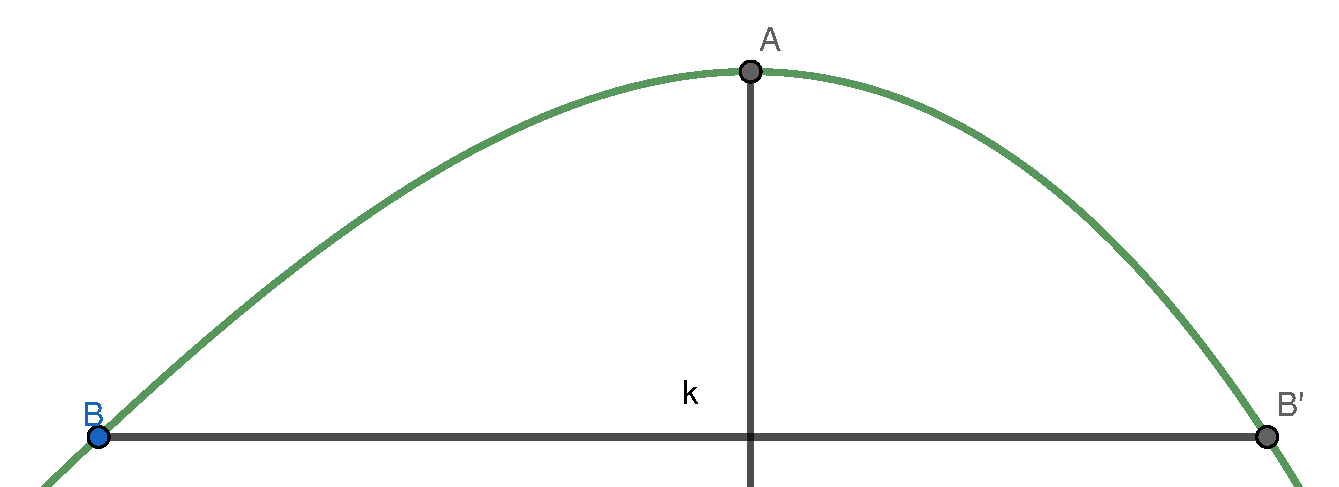
\includegraphics[scale=0.4]{Image/2019.pdf}
        \end{center}
        Ý tưởng của câu này là sẽ xét các đoạn xoay quanh điểm cực trị của $f(x)$ thì với $B < A$ thì luôn tồn tại $B' > A$ sao cho $f(B)  = f(B')$.
        
        
        Ta xét đoạn $[a,b]$ có $a < M < b$ và $c \in (a,M)$ bất kì. Nếu như $[a,b]$ có nhiều hơn một cực trị thì ta chỉ cần co thành đoạn $a' = a + \varepsilon_1 = $ và $b' = b - \varepsilon_2$, với $0 < \varepsilon_1, \varepsilon_2 < M$ đủ lớn sao cho $f'(x) = 0$ có duy nhất nghiệm trên $[a',b']$. Khi này ta xét đến đoạn $[a',b']$. 
        
        
        Không mất tính tổng quát, giả sử đoạn có 1 cực trị $M$ là $[a,b]$, và sẵn theo câu a) thì giả sử $M = max\{f(x)\}$ trên $[a,b]$
        
        
        Đặt $g(x) = f(x) - f(c)$ thì có $g(a) < 0$ và $ g(b) > 0$ thì $g(a).g(b) < 0$, rõ ràng là $g(x)$ có nghiệm trên $(a,b)$, tức là $\exists c' \in (a,b)\backslash{c}$ sao cho $f(c) = f(c')$. 


        Giả sử rằng $c' < M$ thì khi này ta có $f'(c) = f'(c')$, theo định lý Rolle tồn tại $d$ sao cho $f'(d) = 0$, mà $d < M$ vô lý, nên vì vậy $c' \in (M,b)$. 
        
        
        Tương tự như vậy mà vì $f$ liên tục nên có vô hạn $c \in (a,M)$ đồng thời cũng sinh ra vô hạn $c' \in (M,b)$


        Nếu với mỗi $c$ và $c'$ như vậy ta đặt $x_n = c$ và $y_n = c'$ thì sẽ có $f(x_n) = f(y_n)$ với mọi $n \geq 1$. Và ta sẽ xây dựng công thức tổng quát cho $x_n$ và $y_n$.


        Phân hoạch $[a,M]$ thành $n$ đoạn thì mỗi đoạn có độ dài là $\frac{M - a}{n}$,  và ta có dãy $x_1 = a, x_n = x_{n - 1}+ \frac{M - a}{2^n} $. Khi đó đường thẳng $y = f(x_n)$ nằm ngang trên đồ thị và cắt phần $f(x)$ đoạn $(M,b]$ tại một điểm duy nhất là $y_n$.
        
        Nếu $f(a) < f(b)$ thì ta cho $a$ tiến thêm một khoảng nữa là $a'$ sao cho $f(a') > f(b)$. Và giả sử $f(a) > f(b)$.


        Khi này nếu cho $n \to +\infty$ thì $\lim x_n = M$ thì đường thẳng $y$ cũng tịnh tiến lên trên về $(M,f(M))$, chứng tỏ rằng $(y_n)$ cũng tăng và bị chặn. Khi $y$ tiếp xúc $f(x)$ duy nhất tại điểm $(M,f(M))$ trên $[a,b]$ thì cũng là khi $\lim x_n = \lim y_n = M$, và ta hoàn tất chứng minh.
    \end{sol}
    \begin{bt}\vocab{(VMO 2020).}
        Cho dãy số $(x_n)$ xác định bởi: $x_1=1$ và $x_{n+1}=x_n+3\sqrt{x_n} + \frac{n}{\sqrt{x_n}}$,$\forall$n$\ge1$\\
a) Chứng minh rằng lim$\frac{n}{x_n}=0$\\ 
b) Tính lim$\frac{n^2}{x_n}$
    \end{bt}


    \begin{sol}
        a) Vì $x_n$ là dãy dương nên ta có $\frac{n}{x_n} > 0$. Dễ dàng chứng minh $x_n > n^2$ bằng quy nạp. Thì ta có $\frac{n}{x_n} < \frac{1}{n}$. Cho $n \to +\infty$ thì theo nguyên lý kẹp, $\lim\frac{n}{x_n} = 0$ 


        b) Vì $x_n > n^2$ nên $\lim x_n = +\infty$. Áp dụng định lý Stolz ta có 
        \[\lim \frac{n}{\sqrt{x_n}} =\lim \frac{1}{\sqrt{x_{n + 1}} - \sqrt{x_n}} = \lim \frac{\sqrt{x_{n+1}} + \sqrt{x_n}}{x_{n + 1} - x_n} = \lim \frac{\sqrt{x_n + 3\sqrt{x_n} + \frac{n}{\sqrt{x_n}}}+ \sqrt{x_n}}{3\sqrt{x_n} + \frac{n}{\sqrt{x_n}}} \]
        \[
            = \lim \frac{\sqrt{\sqrt{x_n} + \frac{3}{\sqrt{x_n}} + \frac{n}{x_n\sqrt{x_n}}}+ 1}{3 + \frac{n}{x_n}} = \frac{1 + 1}{3} = \frac{2}{3}
        \]
        Vì vậy $\lim\frac{n^2}{x_n} = \frac{4}{9}$
    \end{sol}

    \begin{bt}\vocab{(VMO 2021).}
        Cho dãy số $(x_n)$ xác định bởi $x_1\in (0;\frac{1}{2})$ và $x_{n+1}=3x_n^2-2nx_n^3, n\geq 1$.\\
        a) Chứng minh rằng $(x_n)$ hội tụ về $0$.

        
        b) Với mỗi $n\ge 1$, đặt $y_n=x_1+2x_2+\cdots+n x_n$. Chứng minh rằng $(y_n)$ có giới hạn hữu hạn.
    \end{bt}

    \begin{sol}
        a) Theo bất đẳng thức AM-GM ta có $$|x_{n + 1 }| = |\frac{x_n}{2n}.(2nx_n)\left(3 - 2nx_n\right)| \leq \frac{x_n}{2n}\left(\frac{3 - 2nx_n + 2nx_n}{2}\right)^2 \leq \frac{9}{16}|x_n|, \forall n\geq 2 $$
        Suy ra $|x_{n + 1}| \leq \left(\frac{9}{16}\right)^n x_1$. Chọn $n$ đủ lớn thì có $\lim x_n = 0$


        b) Theo tiêu chuẩn d'Alembert ta xét biểu thức 
        \[D =\lim\frac{(n + 1)x_{n+1}}{nx_n} \leq \lim \frac{9}{16}\frac{n + 1}{n} = \frac{9}{16}\]
        Vì $D < 1$ nên $y_n$ có giới hạn hữu hạn.
    \end{sol}
    \begin{bt}\vocab{(VMO 2022).}
        Cho $a$ là một số thực không âm và dãy số $(u_n)$ được định nghĩa như sau:
$$u_1=6, u_{n+1} = \frac{2n+a}{n} + \sqrt{\frac{n+a}{n}u_n+4}, \forall n \ge 1$$

Với $a \ge 0$, chứng minh rằng tồn tại giới hạn hữu hạn của $(u_n)$.
    \end{bt}

    \begin{sol}
        Dự đoán $\lim u_n = 5$. Bằng quy nạp ta chứng minh được $u_n \geq 5, \forall n \geq 1$. Ta có khai triển như sau:
        \[
            |u_n - 5| \leq |\frac{2n + a}{n} - 2| + |\sqrt{\frac{n+a}{n}u_n+4} -3| \leq \frac{a}{n} + \frac{\frac{n + a}{n}|u_n - 5| + \frac{5a}{n}}{\sqrt{\frac{ n+a}{n}u_n + 4} + 3}
        \]
        \[
            \leq \frac{n + a}{6n}|u_n - 5| + \frac{5a}{6n}
        \]  
        Vì $a$ là cố định nên ta chỉ cần xét từ $n \geq \lfloor a \rfloor $ là được. Ta có 
        \[|u_n - 5| \leq \frac{1}{3}|u_n -5| + y_n, \text{ với } \lim y_n = \lim \frac{5a}{6n} = 0\]
        Áp dụng bổ đề dãy số ta được $\lim x_n = 5$.
    \end{sol}
    %\vocab{Bình luận: } \textit{Bài toán này còn có một cách làm nữa đó là ta sử dụng giải tích tương tự bài dãy số năm 2017, việc trình bày cách 2 sẽ nhường lại cho bạn đọc.}
    \begin{bt}\vocab{(VMO 2023).}
        Xét dãy số $(a_n)$ thỏa mãn $a_1=\dfrac{1}{2}, a_{n+1}=\sqrt[3]{3a_{n+1}-a_n}$ và $0\le a_n\le 1, \forall n\ge 1.$

a. Chứng minh rằng dãy số $(a_n)$ được xác định duy nhất và có giới hạn hữu hạn.

b. Đặt $b_n=(1+2.a_1)(1+2^2a_2)...(1+2^na_n), \forall n\ge 1.$

Chứng minh rằng dãy số $(b_n)$ có giới hạn hữu hạn.
    \end{bt}

    \begin{sol}
        a) Đặt $a_n = 2\sin{\alpha_n}$. Ta có $\sin{\alpha_n} = 3\frac{a_{n + 1}}{2} - \frac{4a_{n + 1}^3}{2^3} \Rightarrow a_{n + 1} = 2\sin{\frac{\alpha_n}{3}}$
        

        Thực hiện truy toán như vậy nếu đặt $a_1 = 2\sin{\alpha}$ thì ta có $a_n = 2\sin{\frac{\alpha}{3^{n-1}}}$
        

        Do đó $(a_n)$ xác định duy nhất và $\lim a_n = 0$


        b) Ta có $\frac{b_{n + 1}}{b_n} = 1 + 2^na_n > 1$ nên $(b_n)$ tăng. Mặt khác, vì $0 < \frac{\alpha}{3^{n-1}} < \frac{\pi}{2}, \forall n \geq 1$.\\ Xét $f(x) = \sin{x} - x$ trên $(0, \frac{\pi}{2})$ có $f'(x) = \cos{x} - 1 \leq 0$ nên $f(x)$ giảm và $f(x) \leq 0$.\\ Do đó ta có đánh giá $$a_n =  2\sin{\frac{\alpha}{3^{n-1}}} \leq \frac{2\alpha}{3^{n-1}}$$
        Khi này viết lại với chú ý $\ln(x + 1) \leq x, \forall x \geq 1$
        \[
            b_n \leq  \prod_{i = 1}^n \left(1 + \frac{2^{i + 1}\alpha}{3^{i - 1}}\right)
            \Leftrightarrow \ln b_n \leq \sum _{i = 1}^n  \left(1 + \frac{2^{i + 1}\alpha}{3^{i - 1}}\right) \leq \sum_{i = 1}^n 6\alpha\frac{2^i}{3^i} = 12\alpha\left(1 - \left(\frac{2}{3}\right)^n\right) \leq 12\alpha
        \]
        Suy ra được $b_n \leq e^{12\alpha}$. Nên theo Weierstrass thì $(b_n)$ hội tụ, hoàn tất chứng minh.
    \end{sol}

    \begin{bt}\vocab{(VMO 2024).}
        Với mỗi số thực $x$, kí hiệu $\lfloor x \rfloor$ là số nguyên lớn nhất không vượt quá $x$.


Dãy số $\{a_n \}_{n=1}^{\infty}$ được định nghĩa bởi $a_n = \frac{1}{4^{\lfloor -\log_4 n \rfloor}}, \forall n \geq 1.$ Đặt $b_n = \frac{1}{n^2} \left( \sum_{k=1}^n a_k - \frac{1}{a_1+a_2} \right).$

a) Tìm đa thức $P(x)$ với hệ số thực sao cho $b_n = P \left( \frac{a_n}{n} \right), \forall n \geq 1$.\\
b) Chứng minh rằng tồn tại một dãy số tăng nghiêm ngặt $\{n_k \}_{k=1}^{\infty}$ của các số nguyên dương sao cho$$\lim_{k \to \infty} b_{n_k} = \frac{2024}{2025}.$$
    \end{bt}

    \begin{sol}
        a) Mỗi lần $n$ tăng gấp 4 lần thì $a_n$ cũng tăng gấp 4 lần, nếu không thì các số hạng kề $a_n$ không đổi. Vậy nên với mỗi $n$, $\exists t: 4^t \leq n \leq 4^{t + 1}$ và $a_n = 4^t$.\\
        Ta để ý rằng $a_1 = 1$, $a_2,a_3,a_4 = 4$, $a_5,a_6,...,a_{16} = 16$ và ta có lập luận rằng cứ mỗi $a_{4^{k-1} + 1},a_{4^{k-1} + 2},...,a_{4^k}$ thì giá trị vẫn giữ nguyên, và cứ một cụm như thế thì sẽ có tổng là $T_k = (4^{k} - (4^{k-1} + 1) + 1)4^k = 12.16^{k-1}$.


        Ta đặt $n = 4^m + r$ trong đó $m$ là số lớn nhất sao cho $4^m \leq n$ và $m,r \in \mathbb{Z}^+$. Tất nhiên là ta được $r = n - a_n$. Khi đó có 
        \[S = \sum_{i = 1}^{4^m + r} a_i = \sum_{i = 1}^{4^m}a_i + \sum_{i = 4^m + 1}^{4^m + r} a_n = 1 + \sum_{i = 0}^{m} T_i + a_n.r = 1 + \sum_{i = 0}^{m} 12.16^{i} + a_n(n - a_n)\]\[ = 1 + 4\frac{16^m - 1}{5}  + na_n - a_n^2 = 1 + \frac{4a_n^2 - 4}{5} +na_n -a_n^2 = -\frac{1}{5}a_n^2 + na_n + \frac{1}{5}\]
        Khi này thay $S$ vào $b_n$ ta được 
        \[b_n = \frac{1}{n^2}\left(S - \frac{1}{5}\right) = -\frac{1}{5}.\frac{a_n^2}{n^2} + \frac{a_n}{n} = P\left(\frac{a_n}{n}\right)\]
        Khi này ta có được $P(x) = -\frac{1}{5}x^2 + x$, hoàn tất câu a).


        b) Để giải quyết được câu b) thì ta hãy tìm hiểu một khái niệm khác trong \vocabf{tiền giải tích (Precalculus)} là \vocabf{Tập hợp trù mật}.

        
        \vocab{- Định nghĩa 9: } Một tập con $A$ trong $X$ được gọi \vocabf{trù mật (hoặc dày đặc)} trong $X$ nếu mọi điểm trong $X$ hoặc là thuộc $X$ hoặc gần tùy ý với một phần tử của $A$.


        Ta có một định lý khá quan trọng như sau:
        \begin{theo}[Định lý trù mật]
            -Với $a < b$ là hai số thực bất kì thì luôn tồn tại số hữu tỉ $q$ sao cho $a < q < b$.
        \end{theo}
        \vocab{Chứng minh: }Đặt $c = b - a > 0$. Khi đó tồn tại số nguyên dương $n$ sao cho $0 < \frac{1}{n} < c$. Điều này không phải hiển nhiên, ta có tiên đề sau
        \begin{theo}[Tiên đề Archimedes]
            -Cho $x,y$ là hai số thực dương, khi đó tồn tại số nguyên dương $m$ sao cho $mx > y$
        \end{theo}
        Cách chứng minh tiền đề này phải dùng đến \vocabf{lý thuyết topo} rất phức tạp nên ta hãy tạm thời thừa nhận nó mà không chứng minh lại.



        Chọn $x = c$ và $y = 1$ thì khẳng định trên đúng. Giờ ta xét các số hữu tỉ dạng $\frac{m}{n}$ với $m \in \mathbb{Z}$ và $n$ nguyên dương cố định. Cũng theo tiên đề Archimedes, luôn tồn tại số hữu tỉ $\frac{m_1}{n} < a$  và số hữu tỉ $\frac{m_2}{n} > b$


        Như vậy ta xét các số hữu tỉ $\frac{m_1}{n}, \frac{m_1 + 1}{n},...\frac{m_2 - 1}{n},\frac{m_2}{n}$. Đặt $p$ là số nguyên lớn nhất sao cho $\frac{p}{n} \leq a$. Khi đó có $a < \frac{p + 1}{n} < b$, hoàn tất chứng minh.


        Mở rộng sang ngôn ngữ dãy số thì điều này cho ta một hệ quả vô cùng quan trọng như sau: 
        \begin{theo}[Hệ quả 1]
            -Nếu $a < b$ là hai số thực dương thì tồn tại vô hạn số hữu tỉ thuộc $(a,b)$. Hay nói cách khác luôn tồn tại dãy $(s_n)$ hữu tỉ với $a < s_n < b, \forall n \geq 1$ và $\lim s_n = L$ với $L$ tùy ý thuộc $(a,b)$.
        \end{theo}
        Và ta còn có thể có một hệ quả thứ hai nữa là
        \begin{theo}[Hệ quả 2]
            -Nếu $(a_n)$ là dãy thực có các phần tử thuộc tập $T$ trù mật trên khoảng nào đó thì tồn tại một dãy $s_n$ nguyên dương tăng ngặt sao cho $\lim a_{s_n} = L$ với $L$ thuộc $T$ tùy ý.
        \end{theo}
        Quay trở lại bài toán, ta có $P(1) = \frac{4}{5} < \frac{2024}{2025} < P(2) = \frac{6}{5}$, cho nên vì tính liên tục của $P$ nên tồn tại $\alpha \in (1,2)$ sao cho $P(\alpha) = \frac{2024}{2025}$. Như vậy bài toán sẽ hoàn tất nếu ta chỉ ra được tập hợp 
        \[T = \left\{\frac{4^{i + 1}}{4^i + r} | i,r \in \mathbb{N}, 0 < q \leq 3.4^i\right\}\]
        trù mật trên $(1,2)$. Với $a < b \in (1,2)$ bất kì thì luôn tồn tại số $i,r$ sao cho $$ a < \frac{4^{i + 1}}{4^i + r} < b \Leftrightarrow \frac{a}{4^{i + 1}} < \frac{1}{4^i + r} < \frac{b}{4^{i + 1}} \Leftrightarrow 4^i(\frac{4}{b} - 1) < r < 4^i(\frac{4}{a} - 1) \Leftrightarrow 4^i(\frac{4}{a} - \frac{4}{b}) > 1$$  nếu chọn $i$ đủ lớn, dẫn tới sự tồn tại của $r$, vậy nên $T$ trù mật trên $(1,2)$. 

        
        
        Viết $n = 4^m + r$ thì ta được $\frac{a_n}{n} = \frac{4^{m + 1}}{4^m + r} \in T$. Theo hệ quả trù mật thì vì đã có $\left(\frac{a_n}{n}\right)$ là dãy hữu tỉ nên phải tồn tại dãy $(n_k)$ nguyên dương tăng ngặt để $\displaystyle \lim_{k \to +\infty}\frac{a_{n_k}}{n_k} = P(\alpha) = \frac{2024}{2025}$, hoàn tất chứng minh.
    \end{sol}
    \begin{bt}\vocab{(OLP 30/4 2024).}
        Cho dãy số $(x_n)$ được xác định bởi $$x_1 = 1, x_{n + 1} = \frac{1 + \sqrt{1 + x_n^2} - x_n}{1 + \sqrt{ 1 + x_n^2} + x_n}$$Chứng minh rằng $(x_n)$ có giới hạn hữu hạn và tìm giới hạn đó.
    \end{bt}

    \begin{sol}
        \vocab{Cách 1: Sử dụng bổ đề dãy số.} Viết lại ta có $x_{n + 1} = \sqrt{x_n^2 + 1} - x_n$. Dự đoán $\lim x_n = \frac{1}{\sqrt{3}}$. Lại có 
        $x_{n + 1} = \frac{1}{\sqrt{x_n^2 + 1} + x_n} > 0$ nên cũng có $x_{n+ 1} \leq 1$
        \[(x_{n + 1} - \frac{1}{\sqrt{3}}) = \sqrt{x_n^2 + 1} - \frac{2}{\sqrt{3}} - (x_n - \frac{1}{\sqrt{3}}) = \frac{(x_n + \frac{1}{\sqrt{3}})(x_n - \frac{1}{\sqrt{3}})}{\sqrt{x_n^2 + 1} + \frac{2}{\sqrt{3}}} \leq (\sqrt{3} - 1)(x_n - \frac{1}{\sqrt{3}})
        \]
        \[\Leftrightarrow |x_{n + 1} - \frac{1}{\sqrt{3}}| \leq (2 - \sqrt{3})|x_n - \frac{1}{\sqrt{3}}|\]
        Áp dụng bổ đề dãy số thì $(x_n)$ có giới hạn hữu hạn và $\lim x_n = \frac{1}{\sqrt{3}}$ 


        \vocab{Cách 2: Sử dụng lượng giác.} Đặt $x_n = \tan{x}$. Ta có 
        \[x_{ n + 1} = \sqrt{\tan^2{x} + 1} - tan{x} = \frac{1}{\cos x} - \tan{x} = \frac{\sin{\frac{\pi}{2}} - \sin{x}}{cos{x}} = \frac{2\cos(\frac{\pi}{4} + \frac{x}{2})\sin(\frac{\pi}{4} -\frac{x}{2})}{\sin(\frac{\pi}{2} - x)}\]
        \[
        = \frac{\cos(\frac{\pi}{4} + \frac{x}{2})}{\cos(\frac{\pi}{4} - \frac{x}{2})} = \tan(\frac{\pi}{4} - \frac{x}{2})
        \]
        Khi đó ta sẽ quy nạp được $x_n = \tan\left(\frac{\pi}{6} + \frac{\pi}{12}\left(-\frac{1}{2}\right)^{n - 1}\right)$. Vậy nên $\lim x_n = \frac{1}{\sqrt{3}}$
    \end{sol}
    
    \begin{bt}\vocab{(Đồng Tháp TST 2024). }
        Cho dãy số thực $(x_n)$ có $x_1 = 2$ và
        \[x_{n + 1} = \frac{n^2- 1}{x_n} + 2, \forall n \geq 1\]


        a) Chứng minh rằng $\lim x_n = +\infty$


        b) Xét dãy $(y_n)$ được xác định bởi
        \[y_n = \frac{x_1}{1.2^1} + \frac{x_2}{2.2^2} + \dots + \frac{x_n}{n.2^n}\]
        Chứng minh rằng $(y_n)$ có giới hạn hữu hạn và $\lim y_n < 2$.
        
    \end{bt}

    \begin{sol}
        a) Ta sẽ chứng minh quy nạp rằng $n \leq x_n \leq n + 1, \forall n \geq 1$. Với $x_1$ thì hiển nhiên đúng, giả sử mệnh đề đúng với $x_n$, ta có 
        \[x_{n + 1} \geq \frac{n^2 - 1}{n + 1} + 2 = n + 1\]
        \[x_{n + 1} \leq \frac{n^2 - 1}{n} + 2 = n - \frac{1}{n} +2 \leq n + 2\]
        Vậy nên mệnh đề quy nạp là đúng. Lại có $x_n \geq n$ nên $\lim x_n = +\infty$.


        b) Dễ thấy rằng $y_n$ là dãy tăng. Trước tiên ta xét chứng minh bxất đẳng thức sau đúng $ 2^{n - 1} > n, \forall n \geq 3$. Xét $f(x) = 2^{x - 1} - x$ trên $[3,+\infty)$ có $f'(x) = \ln2.2^{x - 1} - 1 > 0, \forall n \geq 3$. Vậy nên $f(x)$ tăng và $f(x) > f(3) = 1 > 0$ nên vì vậy $2^n > 2n, \forall n \geq 3$.
        
        
        Áp dụng đánh giá này đồng thời với $ 2^{n - 1} \geq n, \forall n < 3$, ta có 
        $$
        y_n = \sum_{i = 1}^n \frac{x_i}{i.2^i} \leq \sum_{i = 1}^n \frac{i + 1}{i.2^i} = 
        \sum_{i = 1}^n \frac{1}{2^i} + \frac{1}{i.2^i} < 1 - \frac{1}{2^{n}}+ \sum_{i = 1}^n \frac{1}{2i^2}
        $$
        Ta có đẳng thức tổng nghịch đảo bình phương là $\displaystyle \sum_{i = 1}^{\infty} \frac{1}{i^2} = \frac{\pi^2}{6}$, tương đương $\displaystyle \sum_{i = 1}^{n} \frac{1}{i^2} < \frac{\pi^2}{6}, \forall n \geq 1$ nên ta được
        \[y_n \leq 1 + \frac{\pi^2}{12} \]
        Suy ra $(y_n)$ bị chặn trên. Theo Weierstrass thì $(y_n)$ hội tụ và ta có được $\lim y_n \leq 1 + \frac{\pi^2}{12} < 2$
    \end{sol}


 
        
        \subsection{\LARGE \textcolor{dk}{Lời giải}}
    \newpage

\end{itemize}
\end{document}